\chapter{Hardware and Software}\label{cha:hardware}
The goal of this chapter is present the capabilities and limitations of the hardware used in this thesis. The hardware is divided into different sections and are described in moderate detail, for example, how things are connected and how things are controlled.\\
The \abbrROV frame and thrusters were included in a package from Blue Robotics. In addition to the \abbrROV frame, a Raspberry Pi was used as an onboard computer and a HKPilot Mega 2.7  was used as a input/output (\abbrIO) unit, see \Figureref{fig:apm}. The software in the \abbrROV was built on top of \abbrROS.  Instructions for installation of software and operation of the \abbrROV can be found in Appendices~\ref{app:dependencies} and \ref{app:operation}. \abbrROS is an open source operating system for robot applications and is used in the \abbrROV. The operating system provides message passing, hardware abstraction and thus simplifies communication between different computers \citep{ROS}. The message passing in \abbrROS consists of two parties, subscribers and publishers. When a publisher sends a message on a specific topic any subscribers that listens to that topic receives receives the message. \Figureref{fig:rov_scheme} shows a schematic over the \abbrROV components and their connections.

\begin{figure}
	\centering
		\begin{tikzpicture}[auto, thick, node distance=2cm,>=latex',
			 block/.style  = {draw, rectangle,minimum height=3em, minimum width=6em},
			 sum/.style    = {draw, circle, inner sep=0pt, text width=4mm,align=center, node distance=1cm},
			 input/.style  = {coordinate},
			 output/.style = {coordinate},
			 pinstyle/.style = {pin edge={to-,thin,black}}, scale=0.6, every node/.style={transform shape}]
			 
			 \node [block, node distance=5cm] (ws) {Workstation};
			 \node [block, right of=ws, node distance=4cm] (rasp) {Raspberry pi};
			 \node [block, right of=rasp, node distance=4cm] (HkPilot) {HkPilot};
			 \node [block, right of=HkPilot, node distance=4cm] (esc) {ESC};
			 \node [block, below of=esc, node distance=2cm] (thrust) {Thrusters};
			 \node [block, below of=HkPilot] (pressure) {Pressure sensor};
			 \node [block, below of=rasp] (diag) {JST-XH to USB};
			 \node [block, below of=pressure] (bat) {Battery};
			 
			 
			 \draw[<->, thick] (ws) -- node[above]{Cat 6} (rasp);
			 \draw[thick,red] (rasp) -- node[right]{\color{black} \abbrUSB} (diag);
			 \draw[thick,red] (diag.south) -- ++(0,-1.45)-- node[below]{\color{black} JST-XH} (bat.west);
			 \draw[<->, thick,red] (rasp) -- node[above]{\color{black} \abbrUSB} (HkPilot);
			 \draw[<->, thick,red] (HkPilot) -- node[right]{\color{black} $\text{I}^2\text{C}$} (pressure);
			 \draw[->, thick,red] (HkPilot) -- node[above]{\color{black} \abbrPWM} (esc);
			 \draw[thick,red] (esc) -- node[right,align=left]{\color{black} 3.5 mm \\ \color{black} Connector} (thrust);
			 \draw[thick,red] (bat) -| node[right]{\color{black} HXT 4 mm} ++(2,3.8) -|  ($ (esc.west)+(0,-0.2)$);
			 
			 \node[coordinate, above left = 1cm and 0.4cm of rasp](tl){};
			 \node[coordinate, below left = 4.5cm and 0.4cm of rasp](bl){};
			 \node[coordinate, below right = 2.5cm and 1cm of thrust](br){};
			 \node[coordinate, above right = 1cm and 1cm of esc](tr){};
			 
			 \draw[dotted] (tl) -- (bl) -- (br) -- (tr) -- node[below]{ROV} (tl);
		\end{tikzpicture}
	\caption{Schematic of how \abbrROV components communicate (arrows) and how they are powered (red).}
	\label{fig:rov_scheme}
\end{figure} 
\section{BlueROV Package}
\Figureref{fig:rov} shows the BlueRov from Blue Robotics used in this thesis. The BlueROV package includes an acrylic chassi, an acrylic tube, six electronic speed controllers, six Blue Robotics T200 thrusters, cable penetrators and a cradle for mounting of electronics.
\begin{figure}
\centering
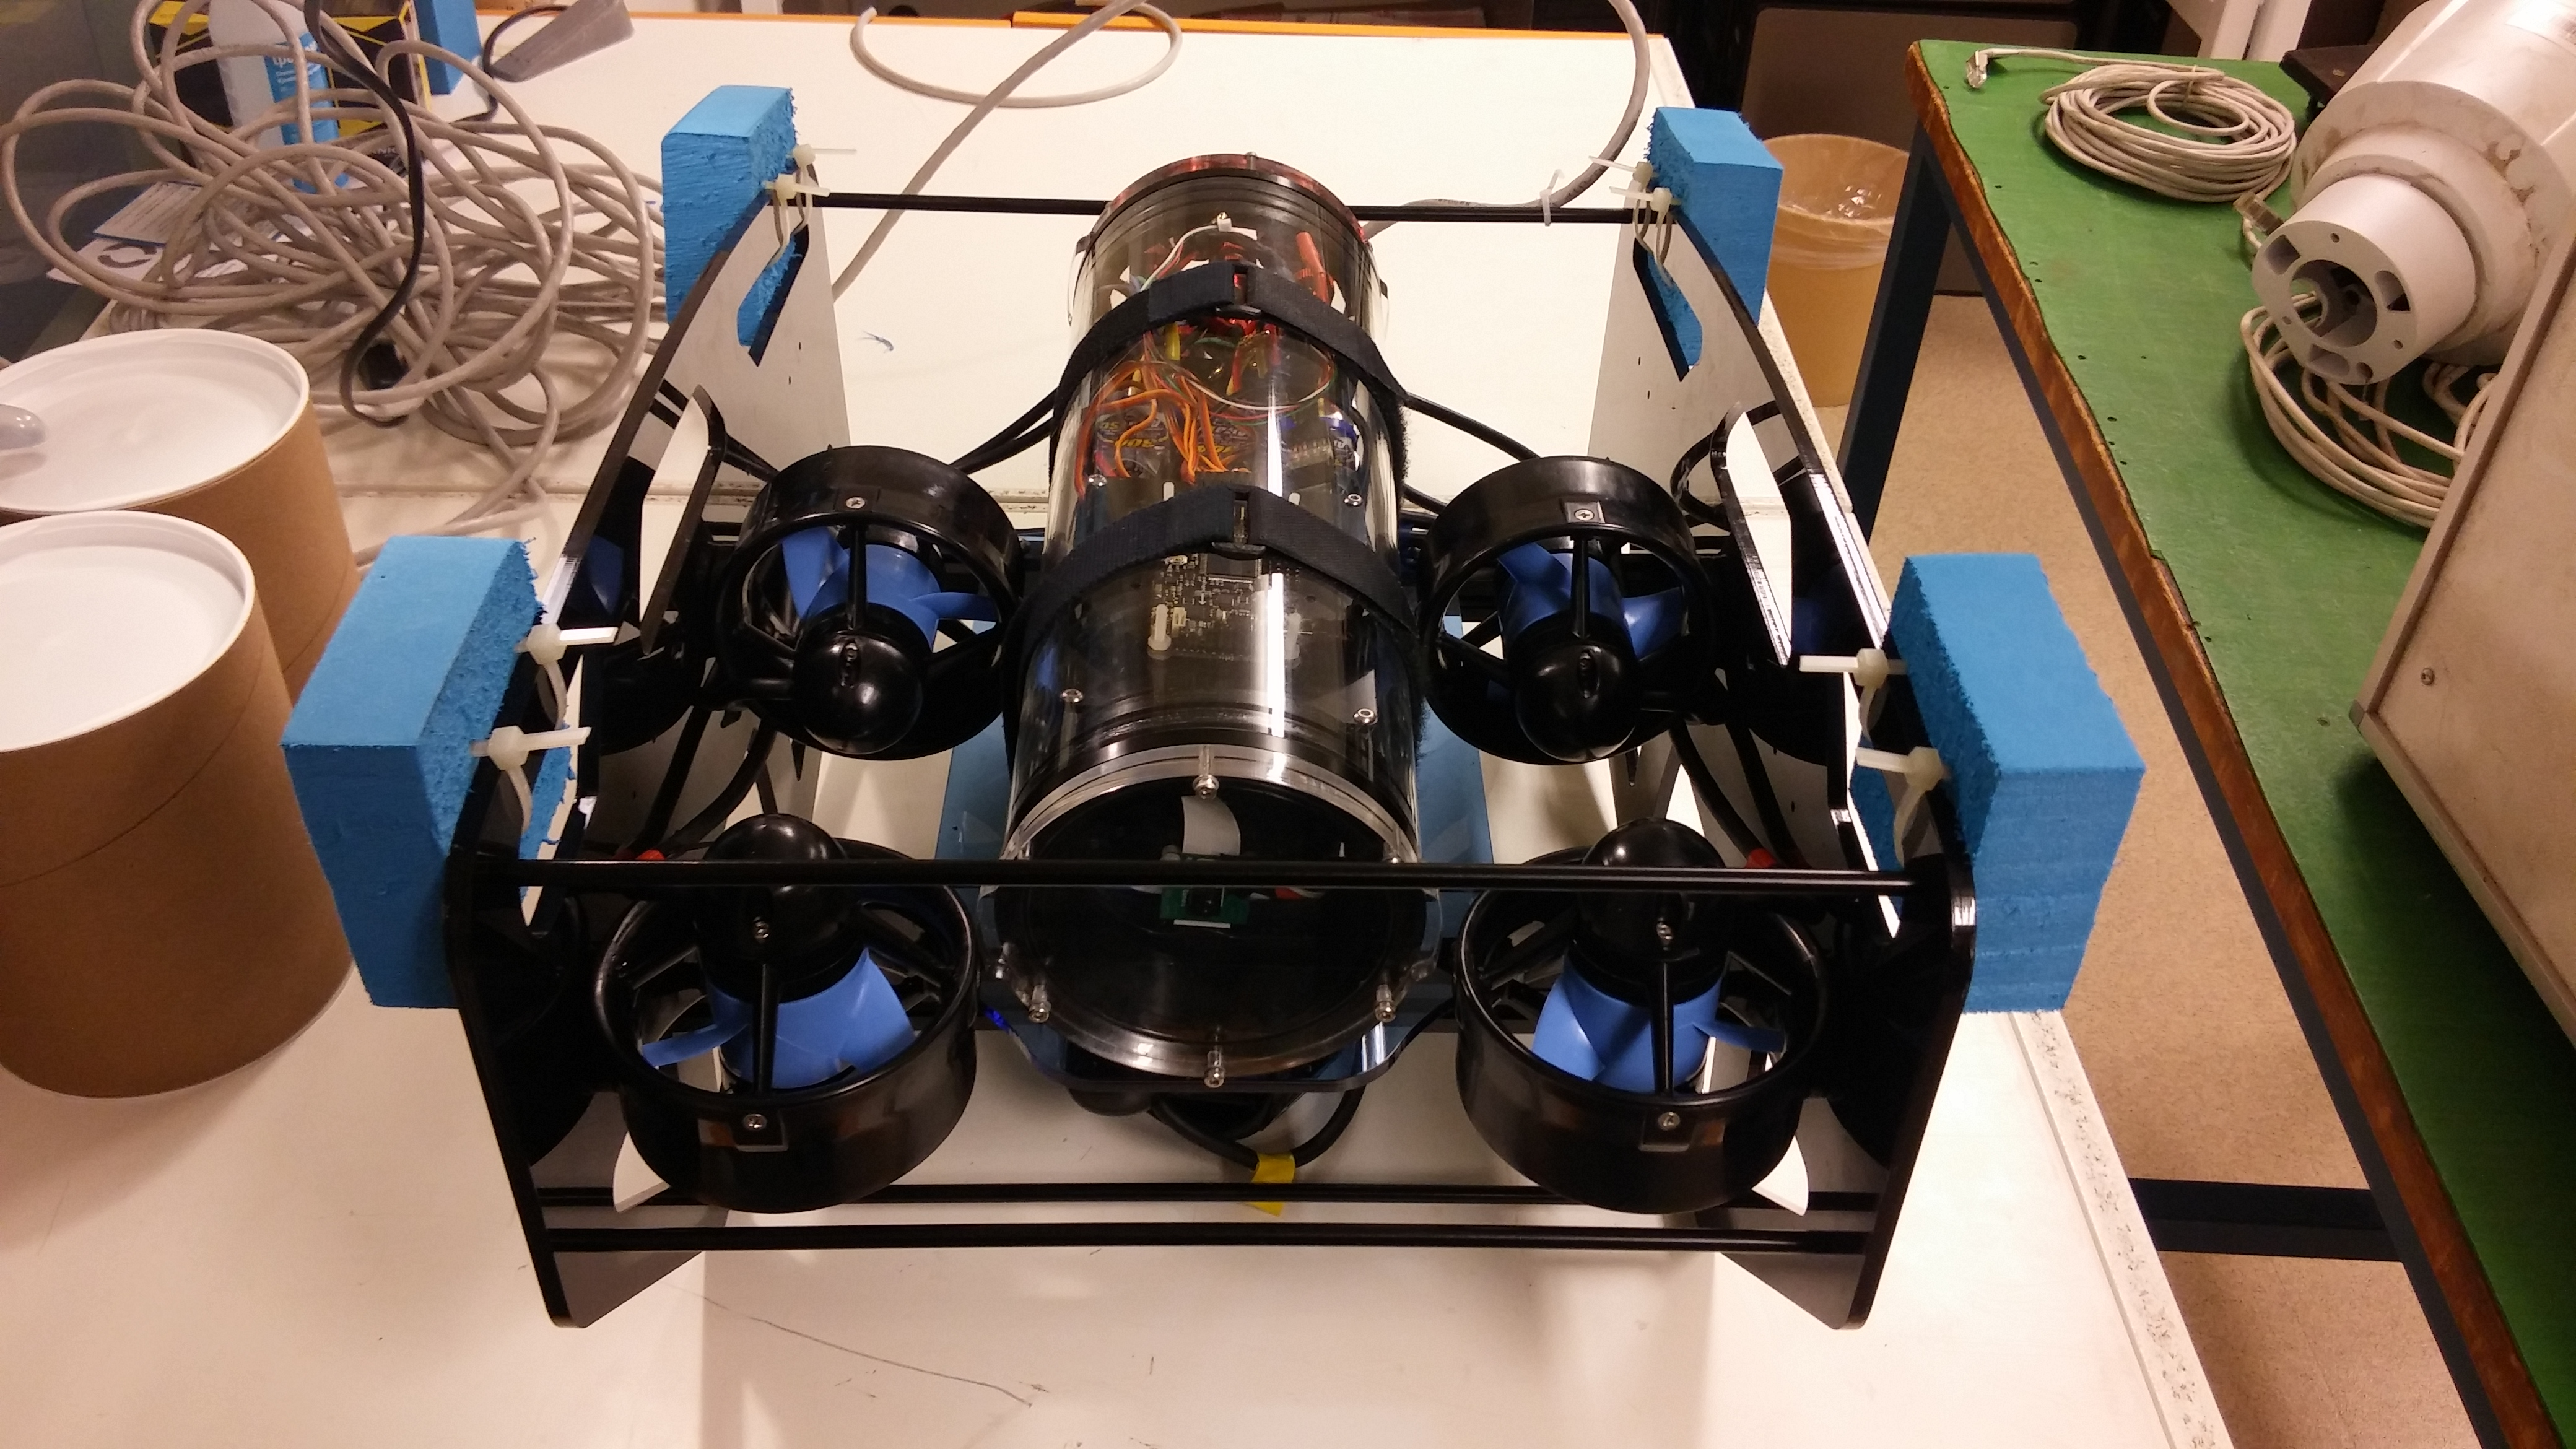
\includegraphics[trim={16cm 5cm 25cm 5cm},clip,width=0.9\textwidth]{rov}
\caption{A frontal view of the BlueRov from Blue Robotics that was used in the thesis.
Note the four blue squares made of EVA foam mounted in the corners for extra buoyancy.}
\label{fig:rov}
\end{figure}

\section{\abbrROV \abbrIO}
The \abbrROV's \abbrIO consists of an HKPilot Mega 2.7 which is based on Ardupilot Mega. The HKPilot Mega 2.7 has the following on chip sensors
\begin{itemize}
    \item Magnetometer - HMC5883L.
    \item Barometer - MS5611-01BA.
    \item Inertial measurement unit (\abbrIMU) - MPU6000.
\end{itemize}
An external pressure sensor MS5837-30BA which was encased in a watertight case by Blue Robotics was connected to the HKPilot Mega 2.7 by \abbrIC.
The HKPilot Mega 2.7 also controls the six \abbrESC:s. The \abbrESC:s are 30A AfroESCs flashed with Blue Robotics linearising firmware. The HKPilot Mega 2.7 is connected to the onboard computer by \abbrUSB cable. The HKPilot Mega 2.7 runs a rosserial-arduino node which is a simpler \abbrROS node that communicates with a master node by serial communication. Scaling and calibration of the sensors are done automatically. However, the offset calibration of the magnetometer has to be performed manually by following the instructions that are produced in the workstation terminal window when the calibration script is run. The external pressure sensor uses the internal barometer to remove the atmospheric pressure offset. The atmospheric pressure offset is measured once, at the start up of the \abbrROV.

\section{Power}
To power the \abbrROV a Turnigy 5000mAh 4S 25C Lipo Pack was used. This is a high discharge battery which ensures that all thrusters can be run at the same time without disruptive voltage drops.
To power the Raspberry Pi 2, a HobbyKing LiPo to \abbrUSB Charging Adapter was used. This adapter connects to the JST-XH connector on the LiPo battery and then outputs regular \abbrUSB voltages and currents. A \abbrUSB to micro-\abbrUSB adapter was used to route the power to the Raspberry Pi. 
The \abbrESC:s are powered via the main lead of the LiPo battery. Lastly, the HKPilot Mega 2.7 is powered via \abbrUSB by the Raspberry Pi \textbf{and} by the \abbrESC:s. 

\section{The Onboard Computer}
The onboard computer was a Raspberry Pi 2 Model B which can be seen in \Figureref{fig:raspberryandcamera}. A Raspicam was connected to the Raspberry Pi 2 and was used to in conjunction with a \abbrROS node to create a video feed. 
The \abbrROS nodes running on the onboard computer can be seen in \Tableref{tab:raspnodes}.
 \begin{table}[tbp]
  \centering
  \caption{\label{tab:raspnodes}%
    The different nodes that run on the onboard computer.}

  \begin{tabular}{l p{0.5\linewidth}}
    \toprule%
    \textbf{Node} & \textbf{Description} \\
    \otoprule%
    roscore             &  Node that handles the \abbrROS backend.\\

    raspicam\_node      &  Camera node for streaming video from the \abbrROV.\\
    
    controller          &  Simulink generated node that can run different controllers.\\
    
    rosserial           &  Serial node for communication with the HKPilot Mega 2.7.\\
    
    matlab\_controller  &  Dynamic reconfigure node for the controller node.\\
    \bottomrule%
  \end{tabular}
\end{table}

\begin{figure}
    \centering
    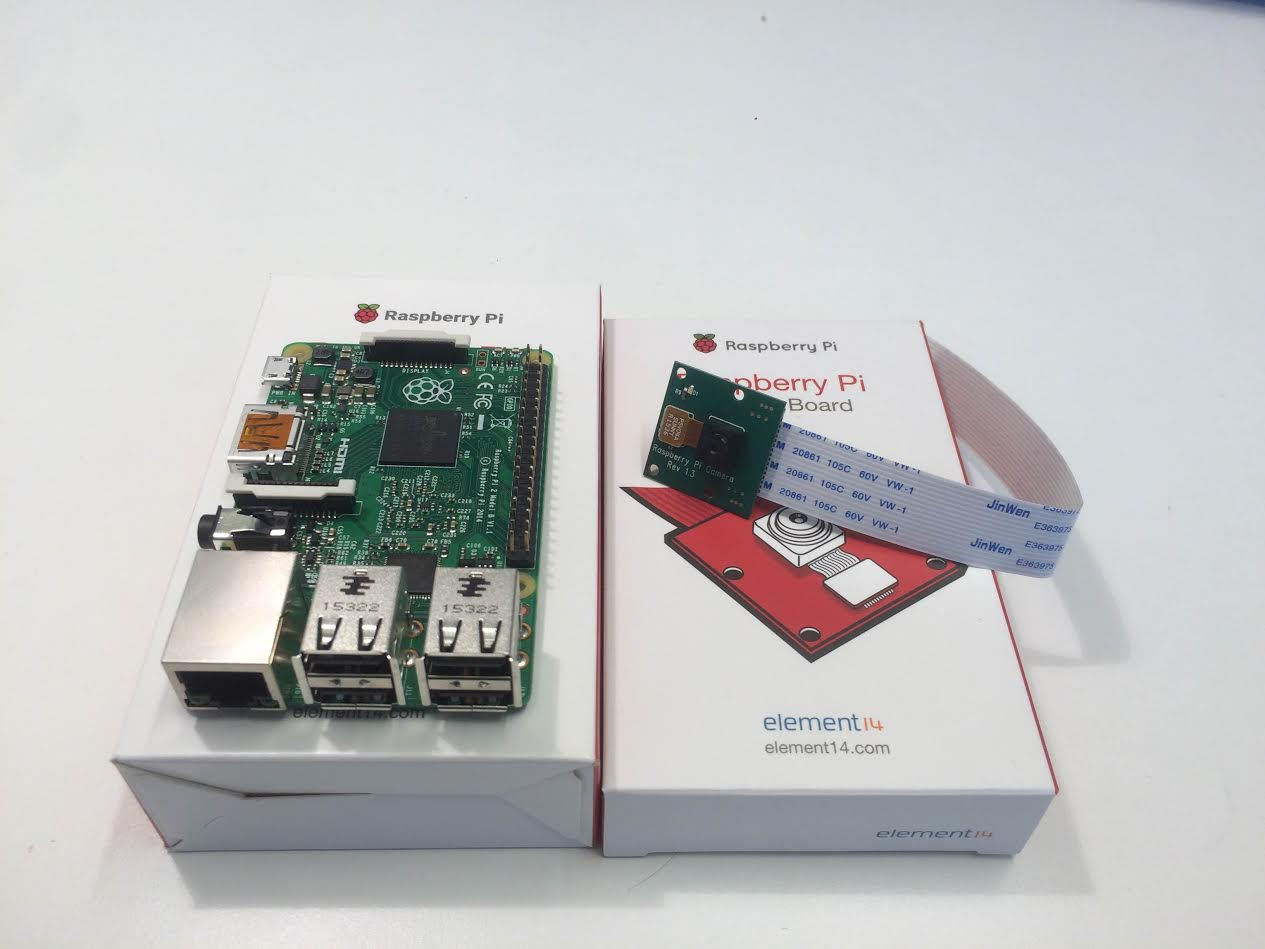
\includegraphics[trim={0 0 0 5cm},clip,width=0.9\textwidth]{raspberryandcamera}
    \caption{The Raspberry Pi 2 Model B, the onboard computer, is shown to the left and the raspicam is shown on the right.}
    \label{fig:raspberryandcamera}
\end{figure}

\begin{figure}
    \centering
    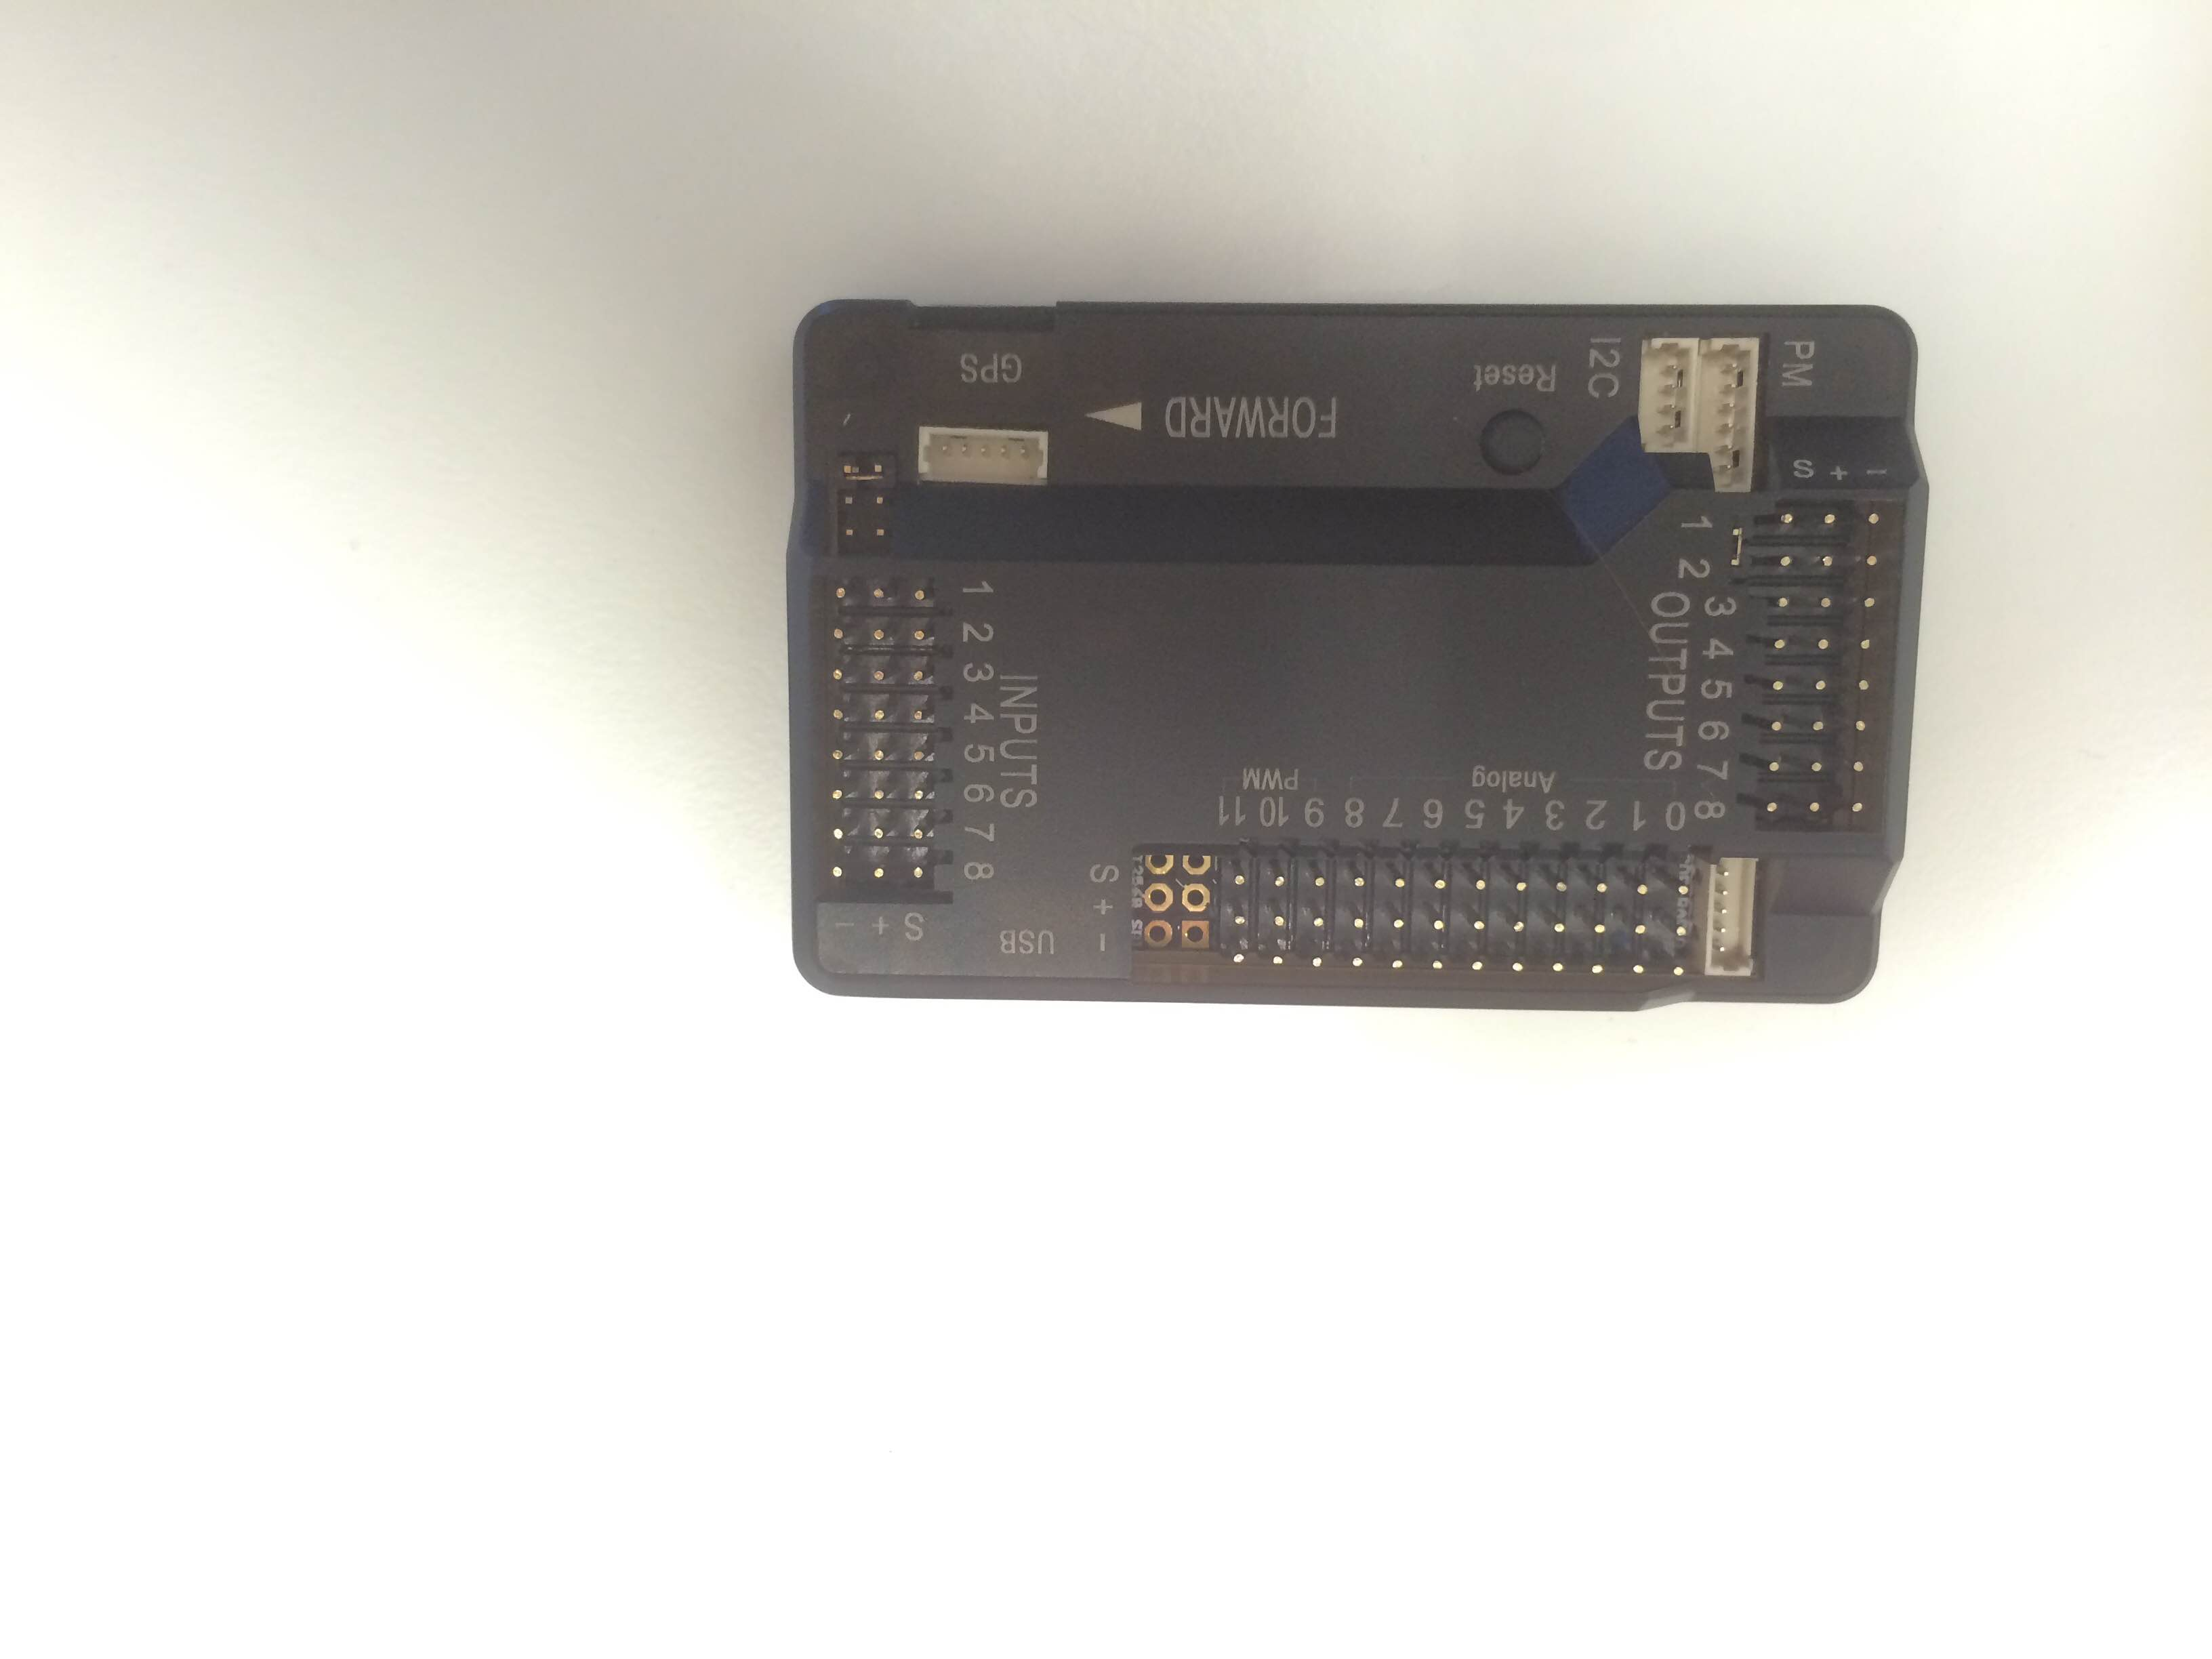
\includegraphics[trim={0 0 4cm 10cm},angle=180,origin=c,clip,width=0.9\textwidth]{apm}
    \caption{The HKPilot Mega 2.7 used for \abbrIO.}
    \label{fig:apm}
\end{figure}

\section{The Workstation}
The workstation used in the thesis is a Lenovo T430 with an Intel\textregistered i5-3210M processor and Intel\textregistered HD Graphics 4000. The workstation was connected via a Cat 6 tether to the Raspberry Pi 2. The different \abbrROS nodes that are run on the workstation can be seen in \Tableref{tab:workstationnodes}.
\begin{table}[tbp]
  \centering
  \caption{\label{tab:workstationnodes}%
    The different node that run on the workstation.}

  \begin{tabular}{l p{0.5\linewidth}}
    \toprule%
    \textbf{Node} & \textbf{Description} \\
    \otoprule%
    heartbeat       & Node for checking the connection with the HKPilot Mega 2.7.\\

    teleop\_xbox    & Xbox node for handling inputs from the xbox controller.\\

    joy             & A joystick node for interacting with the \abbrOS:s \abbrUSB inputs.\\
        
    
    rqt             & A \abbrGUI for the \abbrROV.\\
    
    sensorfusion    & The sensor fusion node. \\
    \bottomrule%
  \end{tabular}
\end{table}